\documentclass[	a4paper,
				12pt,
				parskip,
				openbib,
				toc=bibliography,
				toc=listof,
				toc=index
				]{scrreprt}
\usepackage{blindtext}

\usepackage[T1]{fontenc}
\usepackage{lmodern}

\usepackage[british,UKenglish,USenglish,english,american]{babel}
%\usepackage[ngerman]{babel}

\usepackage{helvet}
\renewcommand{\familydefault}{\sfdefault}

\usepackage{graphicx}
\usepackage{wrapfig}
\usepackage{amsmath}

\usepackage[left=3cm,
			right=2cm,
			top=2.5cm,
			bottom=2cm,
			includeheadfoot]{geometry}
			
        \usepackage{scrhack}
        \usepackage{setspace}
        \linespread{1}

\usepackage[backend=biber, style=verbose-trad3]{biblatex}
\addbibresource{ScPaperTemplate.bib}

\usepackage[hidelinks]{hyperref}


\usepackage{fancyhdr}
\pagestyle{fancy}
\renewcommand{\headrulewidth}{1pt}
\fancyhf{}
\fancyhead[L]{\nouppercase{\leftmark}}
\fancyhead[R]{\thepage}



%\usepackage[toc]{glossaries}
%\usepackage[nottoc]{tocbibind}
%\makeglossaries
%\newglossaryentry{math}
{
        name=mathematic,
        description={is an area of knowledge, which includes the study of such topics as numbers (arithmetic and number theory), formulas and related structures (algebra), shapes and spaces in which they are contained (geometry), and quantities and their changes (calculus and analysis).There is no general consensus about its exact scope or epistemological status.}
}

\newglossaryentry{formula}
{
        name=formula,
        description={A mathematical expression}
}

\newacronym{gcd}{GCD}{Greatest Common Divisor}

\newacronym{lcm}{LCM}{Least Common Multiple}

\begin{document}
%\raggedright
\title{Demo}
\subtitle{Subtitle}
\author{Author}
\date{\today}
\maketitle

\tableofcontents

\chapter{One}
\blindtext \autocite{demo0815}

\section{Image}
\begin{figure}[hbt]
	\centering
  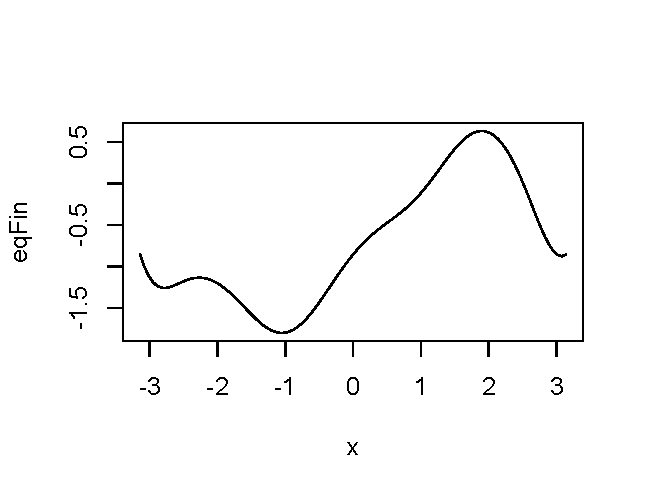
\includegraphics[width=0.5\textwidth]{chapters/one/img/Rplot}
  \caption{Plot}
\end{figure}

\section{Table}
\begin{table}[hbt]
\centering
  \begin{tabular}{l|cc}
    1 & 2 & 3\\
    \hline
    A & B & C\\
    Ä & Ö & Ü
  \end{tabular}
  \caption{Table caption}
\end{table}


\pagebreak
%\printglossary
\listoffigures
\listoftables
\printbibliography

\end{document}